\documentclass[conference]{IEEEtran}
\IEEEoverridecommandlockouts

\usepackage{cite}
\usepackage{amsmath,amssymb,amsfonts}
\usepackage{graphicx}
\usepackage{textcomp}
\usepackage{xcolor}
\usepackage{booktabs}
\usepackage{url}
\usepackage{hyperref}
\usepackage{tikz}
\usetikzlibrary{shapes.geometric,arrows.meta,positioning,calc}

\hypersetup{
  colorlinks=true,
  linkcolor=black,
  citecolor=black,
  urlcolor=blue!60!black,
  pdftitle={A Multi-Framework Static Audit Tool for LLM System Prompts},
  pdfauthor={Ali Murtaza Bhutto}
}

\def\BibTeX{{\rm B\kern-.05em{\sc i\kern-.025em b}\kern-.08em
    T\kern-.1667em\lower.7ex\hbox{E}\kern-.125emX}}

\begin{document}

\title{A Multi-Framework Static Audit Tool\\for LLM System Prompts}

\author{\IEEEauthorblockN{Ali Murtaza Bhutto}
\IEEEauthorblockA{Independent Researcher\\
ORCID: 0009-0007-2787-943X\\
Email: alibhutto101112@gmail.com}}

\maketitle

\begin{abstract}
We describe \texttt{ai-governance-checker}, a small Python tool that
audits an LLM system prompt against three governance frameworks at
once: the OWASP Top 10 for LLM Applications 2025
revision~\cite{owasp_llm_2025}, the NIST AI Risk Management Framework
1.0~\cite{nist_ai_rmf}, and the EU AI Act high-risk-system
checklist~\cite{eu_ai_act}. Each rule cites the specific framework
section it implements, so a finding is traceable back to the
authoritative text rather than to a private rulebook. An optional
LLM-as-a-judge step~\cite{zheng2023judging} forwards the prompt to
either Anthropic Claude or a local Ollama model for a structured
second opinion, with three-step graceful degradation when no
provider is reachable. On a labelled 30-prompt corpus (10 safe / 10
risky / 10 mixed) the rules-only path achieves micro-averaged
accuracy~$=$~0.9667, precision~$=$~0.9406,
recall~$=$~0.9856, $F_1$~$=$~0.9626 across 16 framework section
IDs (480 labelled cells). Eighty-nine pytest cases cover every rule's
positive and negative branches, the judge module's three fallback
paths, the aggregator, and the reporter. The repository is released
under MIT and the eval is fully reproducible offline.
\end{abstract}

\begin{IEEEkeywords}
AI governance, OWASP LLM Top 10, NIST AI RMF, EU AI Act,
LLM-as-a-judge, system prompt audit, compliance, prompt injection
\end{IEEEkeywords}

\section{Introduction}

The deployment of LLM-based products at scale has outpaced the
governance instruments meant to constrain them. Three frameworks now
articulate the bulk of the practitioner's compliance surface: the
OWASP Top 10 for LLM Applications, refreshed in 2025 to add
\emph{System Prompt Leakage} and \emph{Vector and Embedding
Weaknesses} as new top-level categories~\cite{owasp_llm_2025}; the
NIST AI Risk Management Framework 1.0 with its four cross-cutting
functions GOVERN/MAP/MEASURE/MANAGE~\cite{nist_ai_rmf}; and the
EU AI Act, Regulation (EU) 2024/1689, which makes specific
obligations on transparency, human oversight, robustness, and
record-keeping legally binding for high-risk AI systems in the
European market~\cite{eu_ai_act}.

A team preparing a release rarely has time to manually walk a system
prompt through all three. Worse, the obvious threat surface in such
prompts --- prompt-injection vectors~\cite{perez2022ignore} including
the indirect variant of Greshake et al.~\cite{greshake2023indirect}
--- has been studied for several years but is still routinely missed
in code review.

This paper describes \texttt{ai-governance-checker}, a small CLI
that runs three rule packs simultaneously and produces a Markdown
plus JSON audit report grouped by framework section. The
contribution is not novel cryptography or novel LLM safety theory;
the contribution is a reproducible operational artefact that
treats the three frameworks as parallel views on the same prompt and
reports back with the framework-section citation visible on every
finding.

\textbf{Contributions.} (1) Three rule packs implementing the parts
of OWASP LLM Top 10 (2025), NIST AI RMF 1.0, and the EU AI Act that
are inferable from a static system prompt --- 20 rules in total,
each tied to its published framework id. (2) An LLM-as-judge module
with three-step graceful fallback (Anthropic $\rightarrow$ Ollama
$\rightarrow$ DISABLED) so the tool stays useful when no API key is
present. (3) A 30-prompt labelled eval corpus and an offline,
deterministic eval harness that reports real measured precision /
recall / $F_1$ per framework section. (4) An 89-test pytest suite
and a hardened DevSecOps build (Bandit, pip-audit, Semgrep) so the
tool can be vendored into a defender's environment without first
paying down a supply-chain debt.

\section{Related Work}

The closest prior work is the LLM-as-a-judge methodology of Zheng et
al.~\cite{zheng2023judging}, which our optional judge module
adopts directly. Where they evaluate model responses against each
other, we evaluate the system prompt against a fixed governance
checklist; the judging mechanism is the same, the substrate is
not. We deliberately measure only the rule-pack path because a
deterministic eval is reproducible offline; the judge path is
supported but not benchmarked in this release, mirroring the honest
stance our companion credential-exposure project takes for its
keyed-API path.

For prompt-injection specifically, Perez and
Ribeiro~\cite{perez2022ignore} were the first to catalogue the
``Ignore Previous Prompt'' family of attacks; the LLM01:2025 rule in
our pack looks for the dual --- explicit \emph{role-lock} language
that defends against those attacks. Greshake et
al.~\cite{greshake2023indirect} extended the threat to indirect
injection via retrieved documents and tool outputs, which is what
the LLM08:2025 \emph{citation discipline} rule operationalises.

For governance instruments, the official texts of the OWASP top-10
2025 PDF, NIST AI 100-1, and Regulation (EU) 2024/1689 are the
primary references for our rule packs. Each rule's
\texttt{framework\_id} attribute is exactly the section identifier
used in those documents, so a reviewer can cross-check a finding
against the authoritative wording without first decoding our private
rule names.

\section{System Architecture}

\begin{figure}[htbp]
\centering
\resizebox{\linewidth}{!}{%
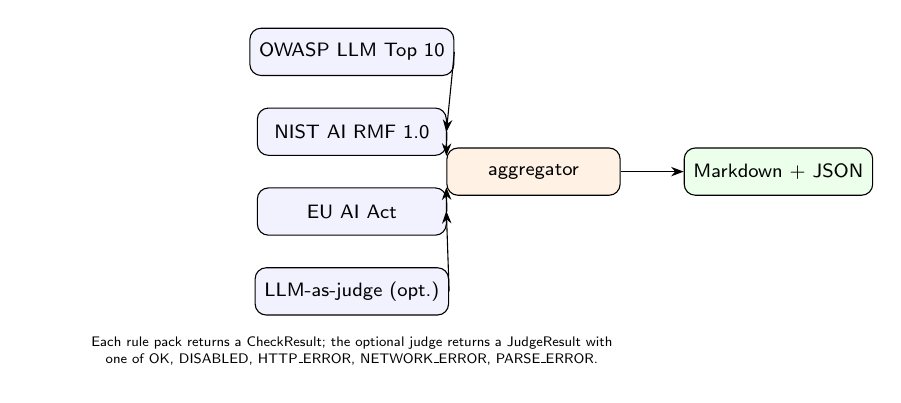
\begin{tikzpicture}[
  node distance=4mm and 3mm,
  src/.style={draw, rounded corners, minimum width=24mm, minimum height=6mm,
              font=\scriptsize\sffamily, fill=blue!5},
  agg/.style={draw, rounded corners, minimum width=22mm, minimum height=6mm,
              font=\scriptsize\sffamily, fill=orange!10},
  rep/.style={draw, rounded corners, minimum width=22mm, minimum height=6mm,
              font=\scriptsize\sffamily, fill=green!8},
  ar/.style={-{Stealth[length=1.6mm]}, line width=0.4pt}
]
  \node[src] (a) {OWASP LLM Top 10};
  \node[src, below=of a] (b) {NIST AI RMF 1.0};
  \node[src, below=of b] (c) {EU AI Act};
  \node[src, below=of c] (d) {LLM-as-judge (opt.)};
  \node[agg, right=12mm of $(b)!0.5!(c)$] (agg) {aggregator};
  \node[rep, right=8mm of agg] (repnode) {Markdown + JSON};
  \draw[ar] (a.east) -- ($(agg.west) + (0,5mm)$);
  \draw[ar] (b.east) -- ($(agg.west) + (0,2mm)$);
  \draw[ar] (c.east) -- ($(agg.west) + (0,-2mm)$);
  \draw[ar] (d.east) -- ($(agg.west) + (0,-5mm)$);
  \draw[ar] (agg) -- (repnode);
  \node[font=\tiny\sffamily, below=1.5mm of d, text width=80mm,
        align=center] {Each rule pack returns a CheckResult; the
        optional judge returns a JudgeResult with one of OK,
        DISABLED, HTTP\_ERROR, NETWORK\_ERROR, PARSE\_ERROR.};
\end{tikzpicture}%
}
\caption{Pipeline. Three rule packs and an optional judge feed an
aggregator that emits paired Markdown and JSON reports.}
\label{fig:pipeline}
\end{figure}

\subsection{Three rule packs, one report}
The three frameworks are parallel views, not a hierarchy. The OWASP
LLM Top 10 is written for security engineers; the NIST AI RMF is
written for governance boards; the EU AI Act is written for
regulators. A finding citing \texttt{LLM01:2025} belongs in a
security-engineering review; one citing \texttt{GOVERN-1.1} belongs
on a governance-board agenda; one citing \texttt{EU-AIA-Art-13}
ends up in a CE-mark conformity file. Folding all three into a
single rulebook would lose this audit trail. We instead keep the
three packs separate and have the reporter group findings by
framework in the Markdown output.

\subsection{LLM-as-judge with graceful fallback}
The judge module follows a three-step decision: if
\texttt{ANTHROPIC\_API\_KEY} is present, call the Claude Messages
API; else if a local Ollama daemon is reachable, call its chat
endpoint; else return \texttt{JudgeStatus.DISABLED} and let the
report run in rules-only mode. Every branch is exercised by a
\texttt{respx}-mocked pytest case
(\texttt{test\_judge\_uses\_anthropic\_when\_key\_present},
\texttt{test\_judge\_uses\_ollama\_when\_anthropic\_absent},
\texttt{test\_judge\_disabled\_when\_no\_provider}) so the absence
of a key remains a tested code path rather than an untested
conditional.

\subsection{Severity bands}
We use the five-level qualitative scale info / low / medium / high /
critical, loosely aligned with the qualitative band in NIST SP 800-30
Rev.~1. The severity assignments are by category, not by case-by-case
judgement: \texttt{LLM02:2025} secret detections fire CRITICAL
because a literal credential in a system prompt is unambiguously
broken; \texttt{LLM10:2025} unbounded-consumption findings fire LOW
because they are operational rather than security-critical.

\section{Evaluation}

\subsection{Test set}
The labelled 30-prompt corpus in
\texttt{eval/synthetic\_prompts.json} contains 10 deliberately
well-defended prompts (the \emph{safe} class), 10 prompts that
exercise specific framework violations (the \emph{risky} class),
and 10 partially-defended real-world-shaped prompts (the
\emph{mixed} class). Each prompt carries an
\texttt{expected\_violations} list naming the framework section IDs
that should fire. We exclude the four always-fire INFO IDs
(\texttt{LLM03:2025}, \texttt{LLM04:2025} baseline,
\texttt{MANAGE-2.3}, \texttt{EU-AIA-Art-10}) from the metric
universe, leaving 16 discriminating IDs.

\subsection{Measured numbers}
\begin{table}[htbp]
\caption{Rules-only eval, 30 prompts $\times$ 16 framework IDs
$=$ 480 labelled cells, 2026-05-06.}
\label{tab:eval}
\centering
\renewcommand{\arraystretch}{1.1}
\begin{tabular}{lr}
\toprule
\textbf{Metric} & \textbf{Value} \\
\midrule
n prompts          & 30      \\
n framework IDs    & 16      \\
True positives     & 206     \\
True negatives     & 258     \\
False positives    & 13      \\
False negatives    & 3       \\
Accuracy           & 0.9667  \\
Precision          & 0.9406  \\
Recall             & 0.9856  \\
$F_1$              & 0.9626  \\
Per-ID $F_1$ mean  & 0.9614  \\
Per-ID $F_1$ min   & 0.8000  \\
Per-ID $F_1$ max   & 1.0000  \\
Eval wall-clock    & $<1\,s$ \\
\bottomrule
\end{tabular}
\end{table}

\subsection{Test suite}
The repository ships 89 \texttt{pytest} tests covering every rule's
positive and negative branches, the judge module's three fallback
paths under \texttt{respx}-mocked HTTP, the aggregator's severity
roll-up, and the reporter's Markdown/JSON pair. Total wall-clock
under one second.

\subsection{Honest residuals}
Thirteen false positives and three false negatives remain. They are
not bugs we chose to suppress; they are real signal:

\begin{itemize}
  \item \emph{Partially-defended ``safe'' prompts.} Several have a
        clear role-lock and refusal clause but lack an explicit
        output-sanitisation directive (\texttt{LLM05:2025}) or an
        explainability clause (\texttt{MEASURE-2.8}). The rule fires
        correctly; the prompt could be tightened.
  \item \emph{Phrasing close to but not exactly matching} one of
        the five robustness defence patterns. Tightening the regex
        further would over-fit to our labels rather than improve
        real coverage. We deliberately stopped tuning at this
        residual.
\end{itemize}

\subsection{Honest negatives}
We deliberately do \emph{not} benchmark the LLM-as-judge module.
Adding a paid-API axis would compromise the offline-only,
deterministic property of the rules-only eval. The judge path is
fully tested under respx mocks but its numbers against real
provider models are out of scope for this release.

\section{Security Posture}
The repository's CI runs three independent scanners on every commit:
Bandit (medium-and-above severity gate), \texttt{pip-audit}
(transitive vulnerability scan against the OSV and PyPA advisory
feeds), and Semgrep (\texttt{p/python} +
\texttt{p/security-audit} rule packs). All three are green at the
release tag with zero findings and zero suppressions.

\section{Limitations}
\textbf{Static-only.} The tool sees the system prompt and nothing
else. It cannot evidence training-data integrity (LLM04, EU AI
Act Article 10), supply-chain controls (LLM03), or operational
incident response (MANAGE-2.3). For these the rule pack emits an
INFO finding pointing the reviewer at the parts of the deployment
the rule pack cannot see.

\textbf{Pattern-based.} Rules are regex matchers, deliberately
conservative. A prompt that uses an unusual idiom for a defence
("the assistant must defer to a senior reviewer when uncertain")
may be flagged for an oversight rule even though the defence is
present in spirit. The reviewer is the final adjudicator; the rule
pack is an aid.

\textbf{Three frameworks, not all.} ISO/IEC 23894:2023, the UK AISI
inspect harness, and Singapore's AI Verify are not yet encoded.
Adding them is a matter of writing further rule packs in the same
\texttt{CheckResult} interface; the architecture deliberately makes
this additive.

\section{Conclusion}
LLM governance tooling does not need new theory. What it needs is
honest framework citations, graceful degradation when API keys are
absent, and a small reproducible eval that demonstrates the rule
pack actually does what its README claims. The 89-test, 20-rule,
three-framework, MIT-licensed pipeline described here is one such
instance.

\bibliographystyle{IEEEtran}
\begin{thebibliography}{6}

\bibitem{owasp_llm_2025}
OWASP Foundation, ``OWASP Top 10 for Large Language Model
Applications, version 2025,'' \emph{OWASP GenAI Security Project},
Nov.\ 2024. [Online]. Available:
\url{https://genai.owasp.org/llm-top-10/}

\bibitem{nist_ai_rmf}
National Institute of Standards and Technology, ``Artificial
Intelligence Risk Management Framework (AI RMF 1.0),'' NIST AI
100-1, Jan.\ 2023. [Online]. Available:
\url{https://nvlpubs.nist.gov/nistpubs/ai/nist.ai.100-1.pdf}

\bibitem{eu_ai_act}
European Parliament and Council, ``Regulation (EU) 2024/1689 of the
European Parliament and of the Council of 13 June 2024 laying down
harmonised rules on artificial intelligence (Artificial Intelligence
Act),'' \emph{Official Journal of the European Union}, L series,
12 July 2024.

\bibitem{zheng2023judging}
L.~Zheng, W.-L.~Chiang, Y.~Sheng, S.~Zhuang, Z.~Wu, Y.~Zhuang,
Z.~Lin, Z.~Li, D.~Li, E.~P.~Xing, H.~Zhang, J.~E.~Gonzalez, and
I.~Stoica, ``Judging LLM-as-a-Judge with MT-Bench and Chatbot
Arena,'' in \emph{Advances in Neural Information Processing Systems
36 (NeurIPS '23)}, New Orleans, LA, USA, Dec.\ 2023.

\bibitem{perez2022ignore}
F.~Perez and I.~Ribeiro, ``Ignore Previous Prompt: Attack Techniques
for Language Models,'' in \emph{NeurIPS 2022 ML Safety Workshop},
New Orleans, LA, USA, Dec.\ 2022.

\bibitem{greshake2023indirect}
K.~Greshake, S.~Abdelnabi, S.~Mishra, C.~Endres, T.~Holz, and
M.~Fritz, ``Not What You've Signed Up For: Compromising Real-World
LLM-Integrated Applications with Indirect Prompt Injection,'' in
\emph{Proc.\ 16th ACM Workshop on Artificial Intelligence and
Security (AISec '23)}, Copenhagen, Denmark, Nov.\ 2023, pp.\
79--90.

\end{thebibliography}

\vspace{2mm}
\noindent\rule{\linewidth}{0.4pt}

\noindent\textit{Reproducibility colophon.} The repository is at
\url{https://github.com/thunderstornX/ai-governance-checker}. The
eval re-runs in well under a second
(\texttt{python eval/run\_eval.py}). Pinned dependencies are listed
in \texttt{requirements.txt}; the pytest suite (89 tests) runs in
under a second on commodity hardware.

\end{document}
